% Introduction

\section{Scope of this study}

A growing number of Australian firms are turning towards open innovation as a competitive strategy. Not only does this allow them to access external knowledge resources, it also enables them to profit from internally developed knowledge by making it available to other firms. However, little is known about the role of tacit knowledge in open innovation. This is surprising considering tacit knowledge guides much of the learning and thought processes that produce novel ideas. This study attempts to fill this gap in understanding by examining tacit knowledge sharing in three open innovation projects. Particular attention is given to how people are motivated to share tacit knowledge and what different patterns of tacit knowledge brokerage reveal about power-relations in each case. \medskip

\section{Background}

\subsection{Need to innovate}

Much of Australia's prosperity stems from its natural advantages in agriculture and mining \citep{leung2016view}. Unfortunately, Australia is losing some of its comparative advantage\footnote{A country enjoys comparative advantage if it (a) can produce some set of goods at lower cost than a foreign country, and (b) is able to trade its relatively cheaper goods with relative cheaper goods produced by the foreign country} due to shrinking demand for it's mineral resources and increased regional competition. Australia can reverse this trend by becoming more innovative. Innovation can lead to the emergence of new industries that deliver long-term economic prosperity. \medskip

Innovation can be defined as the process of implementing new ideas to create value for an organisation \citep{schumpeter1950capitalism}. As long an idea is perceived as new by all those involved, it is an innovation even though it may appear to others as nothing more than an imitation of something that already exists elsewhere \citep{van1986central}. Failure to innovate places a firm’s ability to survive and prosper at risk \citep{bessant2005managing}. \medskip

Though Australia performs particularly well with respect to knowledge creation, it fares poorly when it comes to converting new knowledge into new-to-market innovations. Innovation does not feature strongly in the business strategies of established Australian firms \citep{dodgson2011systems,leung2016view}. This is reflected in the smattering of university-industry collaborations and low number of researchers employed in the business sector compared to other industrialised nations \citep{pettigrew2012australia}. Australia needs to become better at innovation if it wants to secure its long-term economic prosperity. \medskip

\subsection{Trend towards open innovation}

Firms are finding it is becoming harder to compete in the knowledge-based economy\footnote{The term \enquote{knowledge-based economy} refers to the increasing role of knowledge and technology in economic growth.}. Much of this can be attributed to the ever-increasing technical complexity of products, processes, and services that demand levels of knowledge beyond what most firms possess or can develop in a market-relevant time-frame. Many firms are turning towards open innovation to counter this \citep{enkel2009open,bessant2013innovation,stanko2017under}. \medskip

Open innovation is defined as a distributed innovation process based on carefully managed knowledge flows across firm boundaries, using mechanisms as per the firm's business model\footnote{The term \enquote{business model} refers to the design or architecture of the value creation, delivery, and capture mechanisms of a firm \citep{teece2010business}.}. The business model helps a firm determine which inflows of knowledge can fuel innovation, and which knowledge should be released to other organisations \citep{chesbrough2017future}. \medskip 

A firm's dynamic capability refers to its “ability to integrate, build, and reconfigure internal and external competences to address rapidly changing environments” \citep{teece2007explicating}. Open innovation may be construed as a dynamic capability for managing and capturing value from internal and external knowledge resources \citep{lichtenthaler2011open}. 

Key benefits of open innovation include early access to new technology, sharing of risk, reduced costs of development, better customer acceptance of products or services, and enhanced ability to continuously innovate \citep{ye2013exploring}. Because distributed innovation processes are hard to observe and thus imitate, open innovation is also a useful strategy for sustaining competitive advantage \citep{barney1991firm,lichtenthaler2011open}. \medskip

\subsection{Open innovation processes}

Open innovation can be described in terms of inbound, outbound and coupled innovation processes \citep{chesbrough2006beyond,enkel2009open,gassmann2010future}. \emph{Inbound open innovation} enriches a firm’s knowledge base through integrating suppliers, customers and other external actors \citep{xu2013inbound} whereas \emph{outbound open innovation} refers to the commercial exploitation of knowledge that has been developed in-house \citep{de2016knowledge}. \emph{Coupled open innovation} focuses on strategic partnerships that encompass both inbound and outbound innovation processes \citep{spithoven2013open}. Figure \ref{fig:oi_process} illustrates how these processes may work in practice. \medskip

\begin{figure}
	\centering
	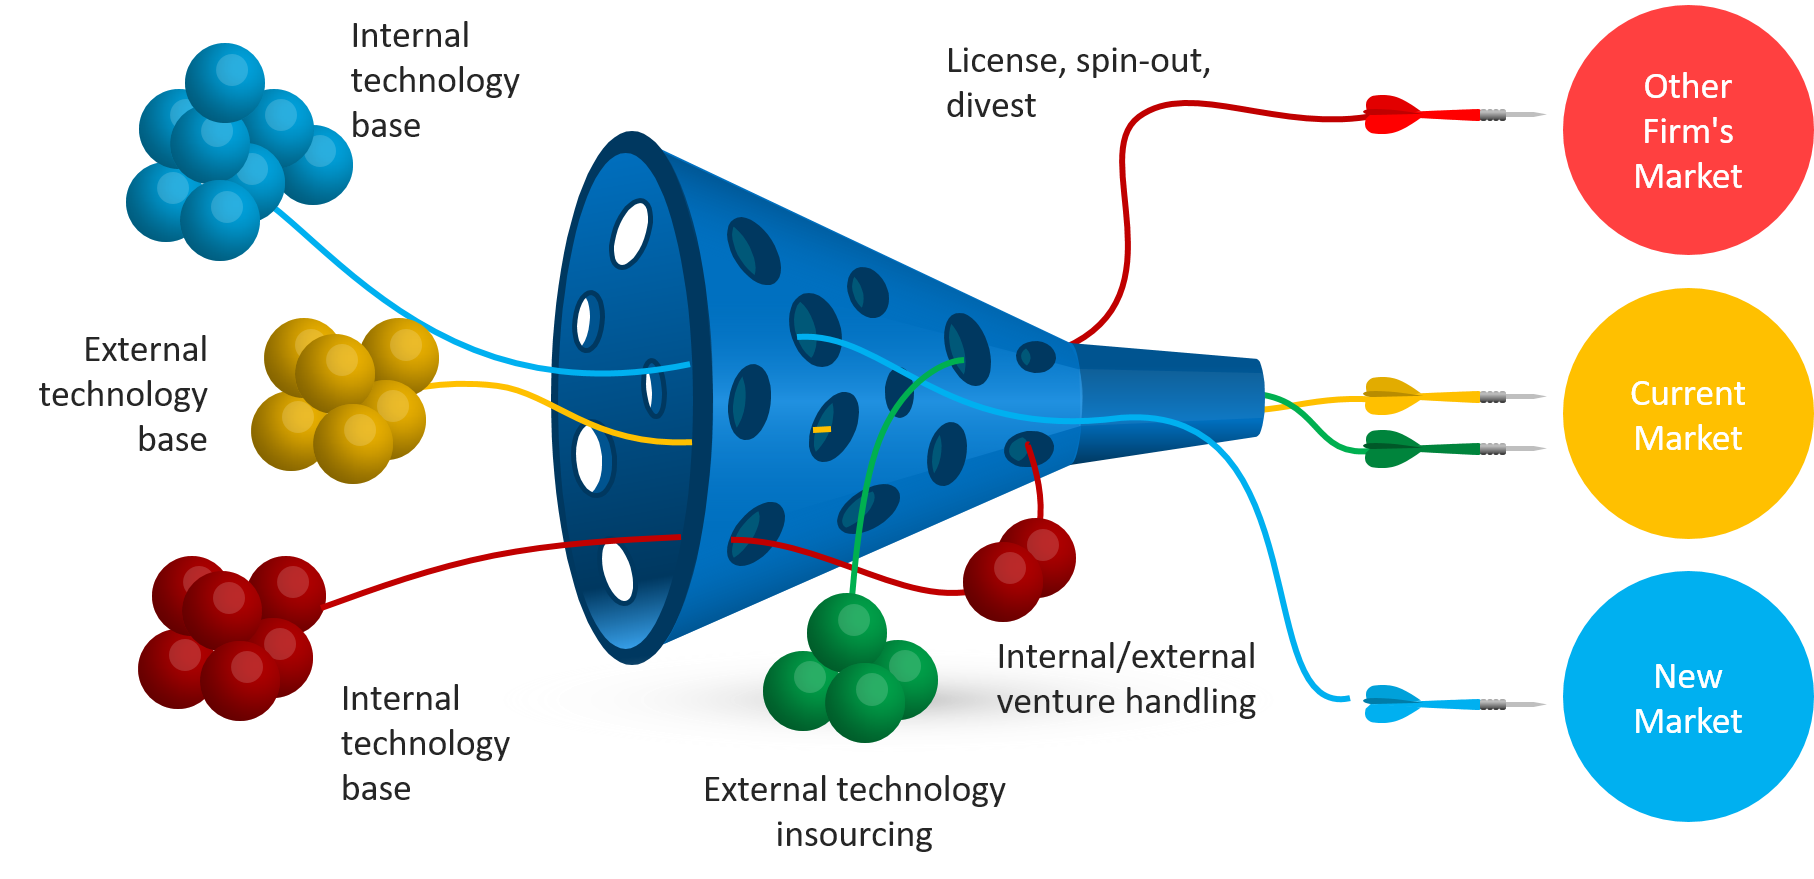
\includegraphics[width=0.9\linewidth]{oi_process_2}
	\caption{Open innovation processes \citep{chesbrough2004open}. Image from SlideModel\texttrademark.}.
	\label{fig:oi_process}
\end{figure}

\subsection{Challenges of open innovation}

Despite its many potential benefits, open innovation presents considerable management challenges \citep{hossain2013open,vanhaverbeke2014surfing}. Overcoming relative differences in absorptive capacity between open innovation partners is a particularly difficult challenge \citep{vanhaverbeke2007connecting,lakemond2016match}. Absorptive capacity refers to the \enquote{ability of a firm to recognise the value of new, external information, assimilate it, and apply it to commercial ends} \citep{cohen1990absorptive}. Firms need absorptive capacity to make sense of new external knowledge and allow them to capture value from open innovation processes \citep{vanhaverbeke2007connecting}. Relative differences in absorptive capacity can impede the flow of knowledge across organisational boundaries, contribute to power imbalances, and undermine alliance performance, all of which can result in sub-optimal open innovation outcomes \citep{szulanski1996exploring,lane1998relative,nooteboom2000learning,vanhaverbeke2007connecting,easterby2008absorptive,phelps2012knowledge}.\medskip 

\subsubsection{Mobilising tacit knowledge}

Past studies of absorptive capacity emphasise the importance of prior knowledge possessed by individuals and groups. The knowledge resource available to a firm can be likened to an iceberg. Explicit knowledge is the visible tip of the iceberg, easy to recognise and access. Hidden beneath the surface of conscious thought, is the vast bulk of the iceberg, symbolising tacit knowledge derived from years of experience, practice, perception, and learning \citep{spender1996making,haldin2000difficulties,mcadam2007exploring,rebernik2007fostering}. Tacit knowledge is associated with terms such as \enquote{intuition}, \enquote{skill}, \enquote{know-how}, and \enquote{expertise} used to describe knowledge that refers to an ability to perform work \citep{horvath2000working,mcadam2007exploring}. Much of the prior knowledge possessed by individuals and groups is likely to be tacit in nature. \medskip

The most common application of tacit knowledge is problem-solving. People with expertise borne from experience not only are able to recognise the situation in which they find themselves in, but also know which actions might be appropriate for dealing with it \citep{simon1971human,leonard1998role}. Tacit knowledge can also used to re-frame problems or anticipate outcomes in intuitive ways \citep{leonard1998role}. Because tacit knowledge guides the thinking that produces novel ideas, it is critical for innovation \citep{leonard1998role,amar2008descriptive}. \medskip

Mobilising tacit knowledge is particularly challenging because people are either unaware of the tacit dimension of their knowledge or unable to express what they know \citep{polanyi1966tacit,leonard1998role}. Many firms do not appreciate the diversity of their knowledge resource and lack processes to unlock the potential value of tacit knowledge \citep{nonaka1994dynamic,horvath2000working}. Sharing tacit knowledge is also something that cannot be mandated. It mostly happens through volition or free will \citep{polanyi1966tacit}. Most employees are inclined to hoard their knowledge to maintain some form of personal advantage \citep{eraut2000non,riege2005three,milne2007motivation}.  \medskip

Tacit knowledge is not transferred but rather interpreted within a specific context \citep{nonaka1995knowledge,duguid2005art,marabelli2014knowing}. Face-to-face social interaction is considered the richest medium because it allows immediate feedback to check understanding and correct interpretations \citep{koskinen2003tacit}. \medskip

\subsubsection{Brokering productive relationships}

Boundary spanners play a key role in open innovation as they broker new relations between otherwise disconnected actors in different organisational networks. More importantly, they facilitate the translation, integration and combination of unfamiliar and distant knowledge \citep{granovetter1973strength,tushman1981boundary,allen1984managing,szulanski2003sticky,burt2004structural,burt2007secondhand,seidler2008use,meyer2010rise,chesbrough2012open}. \medskip

Management efforts to create or widen existing inter-organisational networks may be frustrated by people reluctant to form new ties, facilitate third-party ties, or otherwise change their existing networks \citep{davis2010agency}. Negative attitudes such as \enquote{not-invented-here} and \enquote{not-shared-here} (also referred to as \enquote{not-sold-here}) syndromes can stymie knowledge exchange \citep{lichtenthaler2006attitudes,lichtenthaler2011your,de2014neither,podmetina2015skills,chesbrough2017future}. Not-invented-here syndrome refers to resistance within a firm against externally developed knowledge \citep{katz1982investigating,hussinger2011search,antons2015opening}. Not-shared-here syndrome is a negative attitude towards external exploitation of internally developed knowledge \citep{chesbrough2003open,lichtenthaler2006attitudes,de2014neither}. \medskip

Figuring out ways to overcome negative attitudes towards knowledge sharing is essential to allow the formation of new productive relationships that enable knowledge to be recombined in unique and valuable ways \citep{uzzi1997social,nahapiet1998social,obstfeld2005social,lane2006reification,davis2010agency,meyer2010rise}.\medskip

\section{Research opportunity}

\subsection{Exploring motivational factors}

Tacit knowledge requires significantly more effort than explicit knowledge to communicate. People need to be sufficiently motivated to seek out and share tacit knowledge \citep{leonard1998role}. Past studies show a significant and positive relation between an individual's level of intrinsic motivation and the amount of tacit knowledge they share  \citep[e.g.][]{osterloh2000motivation,kaser2001knowledge,smith2001role}. Intrinsic motivation is about engaging in activity because it is enjoyable or personally meaningful \citep{ryan2000intrinsic}. Although these studies highlight the importance of personal motivation, the psycho-social processes underpinning tacit knowledge sharing and how this impacts open innovation are not well understood. This indicates a need to investigate how personal motivation shapes the development of knowledge sharing relations. \medskip

\subsubsection{Unpacking power-relations}

Though it is often stated that \enquote{knowledge is power}, little attention has been  to power and power-relations in the knowledge management literature \citep{heizmann2015power}. The current power literature is dominated by two contrasting views of power, namely \enquote{power as domination}, also referred to as \enquote{power-over}, and \enquote{power as empowerment}, often characterised as \enquote{power-to} \citep{haugaard2012rethinking}. Sharing tacit knowledge is about empowering others so they can perform work more independently and confidently \citep{bordum2002tacit,lin2007share}. \medskip

The network perspective treats power as inherently relational \citep{ibarra1993network}. How an actor is embedded in a social network either imposes constraints on the actor or presents them with opportunities \citep{burt1992structural,simpson2011network}. Actors with fewer constraints and more opportunities occupy favourable structural positions. Being in a favoured position means that an actor may extract better bargains in exchanges, have greater influence, and be a focus for deference and attention from those in less favoured positions \citep{burt1992structural,hanneman2005introduction,simpson2011network}. \medskip

Actors in knowledge networks serve both as keepers of knowledge and as agents that seek out, communicate, and create knowledge \citep{phelps2012knowledge}. One can assess how actors exercise power by examining patterns of brokerage in knowledge sharing networks. Brokerage may be defined as the \enquote{behaviour by which an actor influences, manages, or facilitates interactions between other actors} \citep{obstfeld2014brokerage}. This definition allows brokerage to be seen in terms of \enquote{power-over} and \enquote{power-to}. \medskip
 
\section{Study objectives}

The extent to which tacit knowledge helps bridge cognitive gaps is poorly understood. Research into brokerage of tacit knowledge is also lacking. This is not surprising, given tacit knowledge is difficult to characterise let alone measure \citep{zander1995knowledge,cavusgil2003tacit}. Tacit knowledge has a significant influence on a firm's absorptive and innovative capacity, and warrants much more attention than it has received so far. \medskip

This study explores tacit knowledge sharing in three open innovation partnerships. Attention is focused on how people are motivated to share tacit knowledge and how tacit knowledge is brokered in each partnership. Four research questions are addressed in this study: \medskip

\begin{description}
    \begin{enumerate}
        \item To what extent does the level and type of personal motivation predict tacit knowledge sharing in open innovation partnerships?
	    \item What does the configuration of tacit knowledge networks reveal about power-relations in open innovation partnerships?
	    \item What is the relationship between tacit knowledge sharing and idea generation in open innovation partnerships?
	   \item How does organisational culture contribute to tacit knowledge sharing in open innovation partnerships
    \end{enumerate}
\end{description}

The study employs social network analysis to (a) assess how individual attributes, such as level and type of personal motivation, educational background, and work experience drive the emergence of tacit knowledge sharing relations, and (b) examine what patterns of brokerage reveal about power-relations in tacit knowledge networks. This analysis is complemented by semi-structured interviews that capture the industrial, organisational, and cultural contexts governing the emergence of collaborative social structures. \medskip  

\section{Research contribution}

This study advances knowledge in two ways. Firstly, the study provides fresh insight into how tacit knowledge sharing facilitates learning and idea generation in open innovation partnerships. Secondly, it breaks new ground by examining how brokerage roles vary according to the amount of tacit knowledge being exchanged and what this means in terms of power-relations. Both contributions should contribute to more effective management of tacit knowledge flows in open innovation. \medskip

\section{Document structure}

This document is organised into nine chapters:

\begin{itemize}[leftmargin=0pt]
  \item[] \textbf{Chapter two} provides an overview of social networks and social network analysis. The reader is introduced to exponential random graph models, an advanced type of social network analysis used in this study..
  
  \item[] \textbf{Chapter three} explores the concept of tacit knowledge and reviews key psychological and social theories that may be used to assess knowledge sharing behaviour. These include the theory of planned behaviour, self-determination theory, structural hole theory, and brokerage theory. The chapter presents a number of propositions that inform the subsequent analysis.
  
  \item[] \textbf{Chapter four} describes the research methodology underpinning this study. This includes explaining the rationale for the convergent parallel mixed method research design used in this study and detailing the quantitative and qualitative procedures used to collect and analyse data.
  
  \item[] \textbf{Chapter five} summarises key characteristics of each open innovation case. This includes a description of the innovation challenge being tackled, information about each partner organisation and the individual actors involved, and a statement on how much progress has been achieved at the time of data collection.
  
  \item[] \textbf{Chapter six} reports on how individual attributes such as level of personal motivation, education level, work location, and job experience shape tacit knowledge sharing relations in each open innovation partnership.
  
  \item[] \textbf{Chapter seven} discusses the different patterns of knowledge brokerage encountered in each partnership and what these reveal about nature power-relations using information from both the social network analysis and semi-structured interviews.
  
  \item[] \textbf{Chapter eight} discusses the implications for managing tacit knowledge flows in open innovation partnerships. 
  
  \item[] \textbf{Chapter nine} summarises the main findings of this study and reflects on some key lessons learned as this study unfolded. This includes describing study limitations and possible avenues for future research. 
\end{itemize}